% !mode::"TeX:UTF-8"
% !TEX program = xelatex
% +-----------------------------------------------------------------------------
% | File: 格式文档
% | 
% |
% | 
% | 
% | Description:
% |   主要是为了方便而设立。  
% |   使用% !mode::"TeX:UTF-8"
% !TEX program = xelatex
% +-----------------------------------------------------------------------------
% | File: 格式文档
% | 
% |
% | 
% | 
% | Description:
% |   主要是为了方便而设立。  
% |   使用% !mode::"TeX:UTF-8"
% !TEX program = xelatex
% +-----------------------------------------------------------------------------
% | File: 格式文档
% | 
% |
% | 
% | 
% | Description:
% |   主要是为了方便而设立。  
% |   使用% !mode::"TeX:UTF-8"
% !TEX program = xelatex
% +-----------------------------------------------------------------------------
% | File: 格式文档
% | 
% |
% | 
% | 
% | Description:
% |   主要是为了方便而设立。  
% |   使用\include{format} 加载本文档
% | 
% | 
% +-----------------------------------------------------------------------------
\documentclass[openany,leqno,11pt]{book}  %ctexart,article

\usepackage{imakeidx}
\usepackage{multicol,multirow} % used for the two-column index 多行多列, 在表格中会用到
\usepackage[bottom]{footmisc}
\usepackage{url}  %这个是加超链接
\usepackage{indentfirst} %首行缩进
\usepackage{bm,amscd,xy,amssymb,amsmath,amsthm,nicefrac,amsfonts,pifont,mathtools,xltxtra}
\usepackage{ctex}
\usepackage{colortbl}
\usepackage{graphicx}
\usepackage{longtable}
\usepackage{booktabs}
% \usepackage{calrsfs} %代数几何中mathcal字体转换 
\usepackage{stmaryrd}% 打\mapsfrom 还有幂级数的符号 \llbracket \rrbracket
% \usepackage{alggp} %代数群文档专用,其中有一些命令由于冲突注销了,如果单独使用,请取消注销

\usepackage{cite} %引用参考文献

%----和后文制作封面一起使用的,如果不通过编译,还是置于后面
%----据说是要放在tikz宏包前面
\usepackage[svgnames]{xcolor} % Required to specify font color

% \newcommand*{\plogo}{\fbox{$\mathcal{PL}$}} % Generic publisher logo %logo 没啥意思

\usepackage{graphicx} % Required for box manipulation
%----
\usepackage{tikz}
	% \usetikzlibrary{cd}
\usepackage{tikz-cd} %xymatrix包文中用过几处, 后来都是在用tikz-cd来画交换图
\xyoption{all}
\newdir{ >}{{}*!/-5pt/@{>}}
% \usepackage{microtype} %microtype 宏包可以改善了单词、字母的间距。它可能做了很多, 但是大部分人察觉不到使用它之后文档的变化。但至少, 加载了 microtype 之后, 文档看起来更好, 也更容易阅读。注意:如果有使用到字体宏包, 需要将 microtype 宏包放在它们的后面, 因为这个宏包对单词、字母的调整和字体是有关的。

\usepackage[pdfencoding=auto,psdextra]{hyperref} % hyperref还是有些小问题,比如section的名字里不能有数学符号,需要用特殊的命令处理掉它。
\usepackage{bookmark}
\renewcommand\bibname{参考文献} %修改bib的名称

%improving spacing in tables (space above and below characters in a row)
\newcommand{\tfix}{\rule{0pt}{2.6ex}}
\newcommand{\bfix}{\rule[-1.2ex]{0pt}{0pt}}

%--一些数学符号, 常用的有\Hom \End \iso(向右箭头上有同构) \id \ker \ima \coker \tor \ext \N \Z \Q \R \mathbb{C}
\newcommand{\Hom}{\mathop{\mathrm{Hom}}} %这个常用
\newcommand{\End}{\mathrm{End}}
\newcommand{\Nil}{\mathrm{Nil}}
\newcommand{\rank}{\mathrm{rank\ }}
\newcommand{\ord}{\mathrm{ord}}
\newcommand{\tr}{\mathrm{tr}}
\newcommand{\id}{\mathrm{id}} %这个常用
\newcommand{\coker}{\mathrm{coker}}
%\newcommand{\ker}{\mathrm{ker}} %\ker直接输入就好
\newcommand{\tor}{\mathrm{Tor}}
\newcommand{\ext}{\mathrm{Ext}}
\newcommand{\ima}{\mathrm{Im}}
\newcommand{\N}{\mathbb{N}}
\newcommand{\Z}{\mathbb{Z}}
\newcommand{\Zn}[1]{\Z/{#1}\Z}
\newcommand{\Q}{\mathbb{Q}}
\newcommand{\R}{\mathbb{R}}
% \newcommand{\C}{\mathbb{C}}  %注销这个的原因是\C 和hyperref宏包冲突。后放弃hyperref,还是有很多冲突,比如页码不对
\newcommand{\F}{\mathbb{F}}

%范畴学常用
\newcommand{\J}{\mathcal{J}}  
\newcommand{\cC}{\mathcal{C}} 
\newcommand{\Top}{\mathbf{Top}}
\newcommand{\Ab}{\mathbf{Ab}}
\newcommand{\Grp}{\mathbf{Grp}}
\newcommand{\Obj}{\mathop{\mathrm{Obj}}}
\newcommand{\sets}{\mathrm{Sets}}
\newcommand*{\colim}{\mathop{\mathrm{colim}}}
\newcommand{\coeq}{\mathrm{coeq}}
\newcommand{\coli}{\colim}

%一些箭头
\newcommand{\iso}{\overset{\cong}{\to}} %isomorphic 这个\to 可以换成\longrightarrow 变长
\newcommand{\weq}{\overset{\sim}{\to}} %表示weak equivalence
\newcommand{\cofi}{\rightarrowtail} %带尾巴的箭头, 单射或者余纤维cofibration
\newcommand{\fib}{\twoheadrightarrow} %满射 或者纤维化fibration
\newcommand{\defo}{\overset{\sim}{\fib}} %这个没用过
\newcommand{\DA}{\Delta} %一般也不用

\def\idem{\mathrm{Idem}}
\renewcommand{\inf}{\rm inf}
\newcommand{\nil}{\rm nil}
\newcommand{\ass}{\mathrm{Ass}}
\newcommand{\der}{\mathrm{Der}}

%Here are some user-defined operators
\newcommand{\Tr}{\operatorname {Tr}}
\newcommand{\GL}{\operatorname {GL}}
\newcommand{\SL}{\operatorname {SL}}

%------这个部分包含了计数器,使得定理,引理等按照同一顺序编号
\newtheorem{theorem}{Theorem}[chapter]
\renewcommand\thetheorem{\arabic{chapter}.\arabic{theorem}} 
\newtheorem{lemma}[theorem]{Lemma}
\renewcommand\thelemma{\arabic{chapter}.\arabic{lemma}} 
\newtheorem{prop}[theorem]{Proposition}
\renewcommand\theprop{\arabic{chapter}.\arabic{prop}} 
\newtheorem{corollary}[theorem]{Corollary}
\renewcommand\thecorollary{\arabic{chapter}.\arabic{corollary}} 
\renewcommand\theequation{\thetheorem}
\newtheorem{conjecture}[theorem]{Conjecture}
\newtheorem*{theorem*}{Theorem}
\newtheorem*{corollary*}{Corollary}
\newtheorem*{lemma*}{Lemma}

%These deal with definition-like environments (i.e., non-italic)
\theoremstyle{definition}
\newtheorem{definition}[theorem]{Definition}
\newtheorem{example}[theorem]{Example}
\newtheorem{remark}[theorem]{Remark}
\newtheorem*{definition*}{Definition}
\newtheorem*{example*}{Example}
\newtheorem*{remark*}{Remark}
\renewcommand\theexample{\arabic{chapter}.\arabic{example}} 

\makeindex
\setlength{\textwidth}{16cm} \setlength{\textheight}{22cm}
\setlength{\oddsidemargin}{0.5cm} \setlength{\topmargin}{0cm}
\setlength{\evensidemargin}{0.5cm} \setlength{\topmargin}{0cm}
% \usepackage[text={150mm,195mm},centering]{geometry}
% \usepackage[body={16cm,24cm}, top=3cm]{geometry}
% 修改列表环境下行间距 2016.3.11
\usepackage{paralist}
\let\itemize\compactitem
\let\enditemize\endcompactitem
\let\enumerate\compactenum
\let\endenumerate\endcompactenum
\let\description\compactdesc
\let\enddescription\endcompactdesc

% \setlength{\pltopsep}{7pt}
% \setlength{\pltopsep}{10pt}

%修改英文字体  这个字体挺好看的 下面两句都是重要的
\usepackage[T1]{fontenc} % The default font encoding only contains Latin characters
\usepackage[noBBpl]{mathpazo} 加载本文档
% | 
% | 
% +-----------------------------------------------------------------------------
\documentclass[openany,leqno,11pt]{book}  %ctexart,article

\usepackage{imakeidx}
\usepackage{multicol,multirow} % used for the two-column index 多行多列, 在表格中会用到
\usepackage[bottom]{footmisc}
\usepackage{url}  %这个是加超链接
\usepackage{indentfirst} %首行缩进
\usepackage{bm,amscd,xy,amssymb,amsmath,amsthm,nicefrac,amsfonts,pifont,mathtools,xltxtra}
\usepackage{ctex}
\usepackage{colortbl}
\usepackage{graphicx}
\usepackage{longtable}
\usepackage{booktabs}
% \usepackage{calrsfs} %代数几何中mathcal字体转换 
\usepackage{stmaryrd}% 打\mapsfrom 还有幂级数的符号 \llbracket \rrbracket
% \usepackage{alggp} %代数群文档专用,其中有一些命令由于冲突注销了,如果单独使用,请取消注销

\usepackage{cite} %引用参考文献

%----和后文制作封面一起使用的,如果不通过编译,还是置于后面
%----据说是要放在tikz宏包前面
\usepackage[svgnames]{xcolor} % Required to specify font color

% \newcommand*{\plogo}{\fbox{$\mathcal{PL}$}} % Generic publisher logo %logo 没啥意思

\usepackage{graphicx} % Required for box manipulation
%----
\usepackage{tikz}
	% \usetikzlibrary{cd}
\usepackage{tikz-cd} %xymatrix包文中用过几处, 后来都是在用tikz-cd来画交换图
\xyoption{all}
\newdir{ >}{{}*!/-5pt/@{>}}
% \usepackage{microtype} %microtype 宏包可以改善了单词、字母的间距。它可能做了很多, 但是大部分人察觉不到使用它之后文档的变化。但至少, 加载了 microtype 之后, 文档看起来更好, 也更容易阅读。注意:如果有使用到字体宏包, 需要将 microtype 宏包放在它们的后面, 因为这个宏包对单词、字母的调整和字体是有关的。

\usepackage[pdfencoding=auto,psdextra]{hyperref} % hyperref还是有些小问题,比如section的名字里不能有数学符号,需要用特殊的命令处理掉它。
\usepackage{bookmark}
\renewcommand\bibname{参考文献} %修改bib的名称

%improving spacing in tables (space above and below characters in a row)
\newcommand{\tfix}{\rule{0pt}{2.6ex}}
\newcommand{\bfix}{\rule[-1.2ex]{0pt}{0pt}}

%--一些数学符号, 常用的有\Hom \End \iso(向右箭头上有同构) \id \ker \ima \coker \tor \ext \N \Z \Q \R \mathbb{C}
\newcommand{\Hom}{\mathop{\mathrm{Hom}}} %这个常用
\newcommand{\End}{\mathrm{End}}
\newcommand{\Nil}{\mathrm{Nil}}
\newcommand{\rank}{\mathrm{rank\ }}
\newcommand{\ord}{\mathrm{ord}}
\newcommand{\tr}{\mathrm{tr}}
\newcommand{\id}{\mathrm{id}} %这个常用
\newcommand{\coker}{\mathrm{coker}}
%\newcommand{\ker}{\mathrm{ker}} %\ker直接输入就好
\newcommand{\tor}{\mathrm{Tor}}
\newcommand{\ext}{\mathrm{Ext}}
\newcommand{\ima}{\mathrm{Im}}
\newcommand{\N}{\mathbb{N}}
\newcommand{\Z}{\mathbb{Z}}
\newcommand{\Zn}[1]{\Z/{#1}\Z}
\newcommand{\Q}{\mathbb{Q}}
\newcommand{\R}{\mathbb{R}}
% \newcommand{\C}{\mathbb{C}}  %注销这个的原因是\C 和hyperref宏包冲突。后放弃hyperref,还是有很多冲突,比如页码不对
\newcommand{\F}{\mathbb{F}}

%范畴学常用
\newcommand{\J}{\mathcal{J}}  
\newcommand{\cC}{\mathcal{C}} 
\newcommand{\Top}{\mathbf{Top}}
\newcommand{\Ab}{\mathbf{Ab}}
\newcommand{\Grp}{\mathbf{Grp}}
\newcommand{\Obj}{\mathop{\mathrm{Obj}}}
\newcommand{\sets}{\mathrm{Sets}}
\newcommand*{\colim}{\mathop{\mathrm{colim}}}
\newcommand{\coeq}{\mathrm{coeq}}
\newcommand{\coli}{\colim}

%一些箭头
\newcommand{\iso}{\overset{\cong}{\to}} %isomorphic 这个\to 可以换成\longrightarrow 变长
\newcommand{\weq}{\overset{\sim}{\to}} %表示weak equivalence
\newcommand{\cofi}{\rightarrowtail} %带尾巴的箭头, 单射或者余纤维cofibration
\newcommand{\fib}{\twoheadrightarrow} %满射 或者纤维化fibration
\newcommand{\defo}{\overset{\sim}{\fib}} %这个没用过
\newcommand{\DA}{\Delta} %一般也不用

\def\idem{\mathrm{Idem}}
\renewcommand{\inf}{\rm inf}
\newcommand{\nil}{\rm nil}
\newcommand{\ass}{\mathrm{Ass}}
\newcommand{\der}{\mathrm{Der}}

%Here are some user-defined operators
\newcommand{\Tr}{\operatorname {Tr}}
\newcommand{\GL}{\operatorname {GL}}
\newcommand{\SL}{\operatorname {SL}}

%------这个部分包含了计数器,使得定理,引理等按照同一顺序编号
\newtheorem{theorem}{Theorem}[chapter]
\renewcommand\thetheorem{\arabic{chapter}.\arabic{theorem}} 
\newtheorem{lemma}[theorem]{Lemma}
\renewcommand\thelemma{\arabic{chapter}.\arabic{lemma}} 
\newtheorem{prop}[theorem]{Proposition}
\renewcommand\theprop{\arabic{chapter}.\arabic{prop}} 
\newtheorem{corollary}[theorem]{Corollary}
\renewcommand\thecorollary{\arabic{chapter}.\arabic{corollary}} 
\renewcommand\theequation{\thetheorem}
\newtheorem{conjecture}[theorem]{Conjecture}
\newtheorem*{theorem*}{Theorem}
\newtheorem*{corollary*}{Corollary}
\newtheorem*{lemma*}{Lemma}

%These deal with definition-like environments (i.e., non-italic)
\theoremstyle{definition}
\newtheorem{definition}[theorem]{Definition}
\newtheorem{example}[theorem]{Example}
\newtheorem{remark}[theorem]{Remark}
\newtheorem*{definition*}{Definition}
\newtheorem*{example*}{Example}
\newtheorem*{remark*}{Remark}
\renewcommand\theexample{\arabic{chapter}.\arabic{example}} 

\makeindex
\setlength{\textwidth}{16cm} \setlength{\textheight}{22cm}
\setlength{\oddsidemargin}{0.5cm} \setlength{\topmargin}{0cm}
\setlength{\evensidemargin}{0.5cm} \setlength{\topmargin}{0cm}
% \usepackage[text={150mm,195mm},centering]{geometry}
% \usepackage[body={16cm,24cm}, top=3cm]{geometry}
% 修改列表环境下行间距 2016.3.11
\usepackage{paralist}
\let\itemize\compactitem
\let\enditemize\endcompactitem
\let\enumerate\compactenum
\let\endenumerate\endcompactenum
\let\description\compactdesc
\let\enddescription\endcompactdesc

% \setlength{\pltopsep}{7pt}
% \setlength{\pltopsep}{10pt}

%修改英文字体  这个字体挺好看的 下面两句都是重要的
\usepackage[T1]{fontenc} % The default font encoding only contains Latin characters
\usepackage[noBBpl]{mathpazo} 加载本文档
% | 
% | 
% +-----------------------------------------------------------------------------
\documentclass[openany,leqno,11pt]{book}  %ctexart,article

\usepackage{imakeidx}
\usepackage{multicol,multirow} % used for the two-column index 多行多列, 在表格中会用到
\usepackage[bottom]{footmisc}
\usepackage{url}  %这个是加超链接
\usepackage{indentfirst} %首行缩进
\usepackage{bm,amscd,xy,amssymb,amsmath,amsthm,nicefrac,amsfonts,pifont,mathtools,xltxtra}
\usepackage{ctex}
\usepackage{colortbl}
\usepackage{graphicx}
\usepackage{longtable}
\usepackage{booktabs}
% \usepackage{calrsfs} %代数几何中mathcal字体转换 
\usepackage{stmaryrd}% 打\mapsfrom 还有幂级数的符号 \llbracket \rrbracket
% \usepackage{alggp} %代数群文档专用,其中有一些命令由于冲突注销了,如果单独使用,请取消注销

\usepackage{cite} %引用参考文献

%----和后文制作封面一起使用的,如果不通过编译,还是置于后面
%----据说是要放在tikz宏包前面
\usepackage[svgnames]{xcolor} % Required to specify font color

% \newcommand*{\plogo}{\fbox{$\mathcal{PL}$}} % Generic publisher logo %logo 没啥意思

\usepackage{graphicx} % Required for box manipulation
%----
\usepackage{tikz}
	% \usetikzlibrary{cd}
\usepackage{tikz-cd} %xymatrix包文中用过几处, 后来都是在用tikz-cd来画交换图
\xyoption{all}
\newdir{ >}{{}*!/-5pt/@{>}}
% \usepackage{microtype} %microtype 宏包可以改善了单词、字母的间距。它可能做了很多, 但是大部分人察觉不到使用它之后文档的变化。但至少, 加载了 microtype 之后, 文档看起来更好, 也更容易阅读。注意:如果有使用到字体宏包, 需要将 microtype 宏包放在它们的后面, 因为这个宏包对单词、字母的调整和字体是有关的。

\usepackage[pdfencoding=auto,psdextra]{hyperref} % hyperref还是有些小问题,比如section的名字里不能有数学符号,需要用特殊的命令处理掉它。
\usepackage{bookmark}
\renewcommand\bibname{参考文献} %修改bib的名称

%improving spacing in tables (space above and below characters in a row)
\newcommand{\tfix}{\rule{0pt}{2.6ex}}
\newcommand{\bfix}{\rule[-1.2ex]{0pt}{0pt}}

%--一些数学符号, 常用的有\Hom \End \iso(向右箭头上有同构) \id \ker \ima \coker \tor \ext \N \Z \Q \R \mathbb{C}
\newcommand{\Hom}{\mathop{\mathrm{Hom}}} %这个常用
\newcommand{\End}{\mathrm{End}}
\newcommand{\Nil}{\mathrm{Nil}}
\newcommand{\rank}{\mathrm{rank\ }}
\newcommand{\ord}{\mathrm{ord}}
\newcommand{\tr}{\mathrm{tr}}
\newcommand{\id}{\mathrm{id}} %这个常用
\newcommand{\coker}{\mathrm{coker}}
%\newcommand{\ker}{\mathrm{ker}} %\ker直接输入就好
\newcommand{\tor}{\mathrm{Tor}}
\newcommand{\ext}{\mathrm{Ext}}
\newcommand{\ima}{\mathrm{Im}}
\newcommand{\N}{\mathbb{N}}
\newcommand{\Z}{\mathbb{Z}}
\newcommand{\Zn}[1]{\Z/{#1}\Z}
\newcommand{\Q}{\mathbb{Q}}
\newcommand{\R}{\mathbb{R}}
% \newcommand{\C}{\mathbb{C}}  %注销这个的原因是\C 和hyperref宏包冲突。后放弃hyperref,还是有很多冲突,比如页码不对
\newcommand{\F}{\mathbb{F}}

%范畴学常用
\newcommand{\J}{\mathcal{J}}  
\newcommand{\cC}{\mathcal{C}} 
\newcommand{\Top}{\mathbf{Top}}
\newcommand{\Ab}{\mathbf{Ab}}
\newcommand{\Grp}{\mathbf{Grp}}
\newcommand{\Obj}{\mathop{\mathrm{Obj}}}
\newcommand{\sets}{\mathrm{Sets}}
\newcommand*{\colim}{\mathop{\mathrm{colim}}}
\newcommand{\coeq}{\mathrm{coeq}}
\newcommand{\coli}{\colim}

%一些箭头
\newcommand{\iso}{\overset{\cong}{\to}} %isomorphic 这个\to 可以换成\longrightarrow 变长
\newcommand{\weq}{\overset{\sim}{\to}} %表示weak equivalence
\newcommand{\cofi}{\rightarrowtail} %带尾巴的箭头, 单射或者余纤维cofibration
\newcommand{\fib}{\twoheadrightarrow} %满射 或者纤维化fibration
\newcommand{\defo}{\overset{\sim}{\fib}} %这个没用过
\newcommand{\DA}{\Delta} %一般也不用

\def\idem{\mathrm{Idem}}
\renewcommand{\inf}{\rm inf}
\newcommand{\nil}{\rm nil}
\newcommand{\ass}{\mathrm{Ass}}
\newcommand{\der}{\mathrm{Der}}

%Here are some user-defined operators
\newcommand{\Tr}{\operatorname {Tr}}
\newcommand{\GL}{\operatorname {GL}}
\newcommand{\SL}{\operatorname {SL}}

%------这个部分包含了计数器,使得定理,引理等按照同一顺序编号
\newtheorem{theorem}{Theorem}[chapter]
\renewcommand\thetheorem{\arabic{chapter}.\arabic{theorem}} 
\newtheorem{lemma}[theorem]{Lemma}
\renewcommand\thelemma{\arabic{chapter}.\arabic{lemma}} 
\newtheorem{prop}[theorem]{Proposition}
\renewcommand\theprop{\arabic{chapter}.\arabic{prop}} 
\newtheorem{corollary}[theorem]{Corollary}
\renewcommand\thecorollary{\arabic{chapter}.\arabic{corollary}} 
\renewcommand\theequation{\thetheorem}
\newtheorem{conjecture}[theorem]{Conjecture}
\newtheorem*{theorem*}{Theorem}
\newtheorem*{corollary*}{Corollary}
\newtheorem*{lemma*}{Lemma}

%These deal with definition-like environments (i.e., non-italic)
\theoremstyle{definition}
\newtheorem{definition}[theorem]{Definition}
\newtheorem{example}[theorem]{Example}
\newtheorem{remark}[theorem]{Remark}
\newtheorem*{definition*}{Definition}
\newtheorem*{example*}{Example}
\newtheorem*{remark*}{Remark}
\renewcommand\theexample{\arabic{chapter}.\arabic{example}} 

\makeindex
\setlength{\textwidth}{16cm} \setlength{\textheight}{22cm}
\setlength{\oddsidemargin}{0.5cm} \setlength{\topmargin}{0cm}
\setlength{\evensidemargin}{0.5cm} \setlength{\topmargin}{0cm}
% \usepackage[text={150mm,195mm},centering]{geometry}
% \usepackage[body={16cm,24cm}, top=3cm]{geometry}
% 修改列表环境下行间距 2016.3.11
\usepackage{paralist}
\let\itemize\compactitem
\let\enditemize\endcompactitem
\let\enumerate\compactenum
\let\endenumerate\endcompactenum
\let\description\compactdesc
\let\enddescription\endcompactdesc

% \setlength{\pltopsep}{7pt}
% \setlength{\pltopsep}{10pt}

%修改英文字体  这个字体挺好看的 下面两句都是重要的
\usepackage[T1]{fontenc} % The default font encoding only contains Latin characters
\usepackage[noBBpl]{mathpazo} 加载本文档
% | 
% | 
% +-----------------------------------------------------------------------------
\documentclass[openany,leqno,11pt]{book}  %ctexart,article

\usepackage{imakeidx}
\usepackage{multicol,multirow} % used for the two-column index 多行多列, 在表格中会用到
\usepackage[bottom]{footmisc}
\usepackage{url}  %这个是加超链接
\usepackage{indentfirst} %首行缩进
\usepackage{bm,amscd,xy,amssymb,amsmath,amsthm,nicefrac,amsfonts,pifont,mathtools,xltxtra}
\usepackage{ctex}
\usepackage{colortbl}
\usepackage{graphicx}
\usepackage{longtable}
\usepackage{booktabs}
\usepackage{calrsfs} %代数几何中mathcal字体转换 
\usepackage{stmaryrd}% 打\mapsfrom
% \usepackage{alggp} %代数群文档专用,其中有一些命令由于冲突注销了,如果单独使用,请取消注销

\usepackage{cite} %引用参考文献

%----和后文制作封面一起使用的,如果不通过编译,还是置于后面
%----举火是要放在tikz宏包前面
\usepackage[svgnames]{xcolor} % Required to specify font color

% \newcommand*{\plogo}{\fbox{$\mathcal{PL}$}} % Generic publisher logo %logo 没啥意思

\usepackage{graphicx} % Required for box manipulation
%----
\usepackage{tikz}
	% \usetikzlibrary{cd}
\usepackage{tikz-cd} %xymatrix包文中用过几处, 后来都是在用tikz-cd来画交换图
\xyoption{all}
\newdir{ >}{{}*!/-5pt/@{>}}
% \usepackage{microtype} %microtype 宏包可以改善了单词、字母的间距。它可能做了很多, 但是大部分人察觉不到使用它之后文档的变化。但至少, 加载了 microtype 之后, 文档看起来更好, 也更容易阅读。注意:如果有使用到字体宏包, 需要将 microtype 宏包放在它们的后面, 因为这个宏包对单词、字母的调整和字体是有关的。

\usepackage[pdfencoding=auto,psdextra]{hyperref} % hyperref还是有些小问题,比如section的名字里不能有数学符号,需要用特殊的命令处理掉它。
\usepackage{bookmark}
\renewcommand\bibname{References} %修改bib的名称

%improving spacing in tables (space above and below characters in a row)
\newcommand{\tfix}{\rule{0pt}{2.6ex}}
\newcommand{\bfix}{\rule[-1.2ex]{0pt}{0pt}}

%--一些数学符号, 常用的有\Hom \End \iso(向右箭头上有同构) \id \ker \ima \coker \tor \ext \N \Z \Q \R \mathbb{C}
\newcommand{\Hom}{\mathop{\mathrm{Hom}}} %这个常用
\newcommand{\End}{\mathrm{End}}
\newcommand{\Nil}{\mathrm{Nil}}
\newcommand{\rank}{\mathrm{rank}}
\newcommand{\tr}{\mathrm{tr}}
\newcommand{\id}{\mathrm{id}} %这个常用
\newcommand{\coker}{\mathrm{coker}}
%\newcommand{\ker}{\mathrm{ker}} %\ker直接输入就好
\newcommand{\tor}{\mathrm{Tor}}
\newcommand{\ext}{\mathrm{Ext}}
\newcommand{\ima}{\mathrm{Im}}
\newcommand{\N}{\mathbb{N}}
\newcommand{\Z}{\mathbb{Z}}
\newcommand{\Zn}[1]{\Z/{#1}\Z}
\newcommand{\Q}{\mathbb{Q}}
\newcommand{\R}{\mathbb{R}}
% \newcommand{\C}{\mathbb{C}}  %注销这个的原因是\C 和hyperref宏包冲突。后放弃hyperref,还是有很多冲突,比如页码不对
\newcommand{\F}{\mathbb{F}}

%范畴学常用
\newcommand{\J}{\mathcal{J}}  
\newcommand{\cC}{\mathcal{C}} 
\renewcommand{\top}{\rm top}
\newcommand{\ab}{\mathfrak{Ab}}
\newcommand{\Grp}{\mathfrak{Grp}}
\renewcommand{\mod}{{\rm Mod}}
\newcommand{\Obj}{\mathop{\mathrm{Obj}}}
\newcommand{\sets}{\mathrm{Sets}}
\newcommand*{\colim}{\mathop{\mathrm{colim}}}
\newcommand{\coeq}{\mathrm{coeq}}
\newcommand{\coli}{\colim}

%一些箭头
\newcommand{\iso}{\overset{\cong}{\to}} %isomorphic 这个\to 可以换成\longrightarrow 变长
\newcommand{\weq}{\overset{\sim}{\to}} %表示weak equivalence
\newcommand{\cofi}{\rightarrowtail} %带尾巴的箭头, 单射或者余纤维cofibration
\newcommand{\fib}{\twoheadrightarrow} %满射 或者纤维化fibration
\newcommand{\defo}{\overset{\sim}{\fib}} %这个没用过
\newcommand{\DA}{\Delta} %一般也不用

\def\idem{\mathrm{Idem}}
\renewcommand{\inf}{\rm inf}
\newcommand{\nil}{\rm nil}
\newcommand{\ass}{\mathfrak{Ass}}
\newcommand{\der}{\mathrm{Der}}

%Here are some user-defined operators
\newcommand{\Tr}{\operatorname {Tr}}
\newcommand{\GL}{\operatorname {GL}}
\newcommand{\SL}{\operatorname {SL}}

%------这个部分包含了计数器,使得定理,引理等按照同一顺序编号
\newtheorem{theorem}{Theorem}[chapter]
\renewcommand\thetheorem{\arabic{chapter}.\arabic{theorem}} 
\newtheorem{lemma}[theorem]{Lemma}
\renewcommand\thelemma{\arabic{chapter}.\arabic{lemma}} 
\newtheorem{prop}[theorem]{Proposition}
\renewcommand\theprop{\arabic{chapter}.\arabic{prop}} 
\newtheorem{corollary}[theorem]{Corollary}
\renewcommand\thecorollary{\arabic{chapter}.\arabic{corollary}} 
\renewcommand\theequation{\thetheorem}
\newtheorem{conjecture}[theorem]{Conjecture}
\newtheorem*{theorem*}{Theorem}
\newtheorem*{corollary*}{Corollary}
\newtheorem*{lemma*}{Lemma}

%These deal with definition-like environments (i.e., non-italic)
\theoremstyle{definition}
\newtheorem{definition}[theorem]{Definition}
\newtheorem{example}[theorem]{Example}
\newtheorem{remark}[theorem]{Remark}
\newtheorem*{definition*}{Definition}
\newtheorem*{example*}{Example}
\newtheorem*{remark*}{Remark}
\renewcommand\theexample{\arabic{chapter}.\arabic{example}} 

\makeindex
\setlength{\textwidth}{15cm} \setlength{\textheight}{22cm}
\setlength{\oddsidemargin}{0.5cm} \setlength{\topmargin}{0cm}
\setlength{\evensidemargin}{0.5cm} \setlength{\topmargin}{0cm}
% \usepackage[text={150mm,195mm},centering]{geometry}

% 制作封面


%----------------------------------------------------------------------------------------
%	TITLE PAGE
%----------------------------------------------------------------------------------------


\newcommand*{\rotrt}[1]{\rotatebox{90}{#1}} % Command to rotate right 90 degrees
\newcommand*{\rotlft}[1]{\rotatebox{-90}{#1}} % Command to rotate left 90 degrees

\newcommand*{\titleBC}{\begingroup % Create the command for including the title page in the document
\centering % Center all text
\def\CP{\textit{\Huge 代数$K$理论讨论班笔记}} % Title
\settowidth{\unitlength}{\CP} % Set the width of the curly brackets to the width of the title
{\color{LightGoldenrod}\resizebox*{\unitlength}{\baselineskip}{\rotrt{$\}$}}} \\[\baselineskip] % Print top curly bracket
\textcolor{Sienna}{\CP} \\[\baselineskip] % Print title

{\color{RosyBrown}\Large 中国科学院大学~~数学科学学院} \\ % Tagline or further description
{\color{RosyBrown}\Large \kaishu{张浩}}\\
{\color{LightGoldenrod}\resizebox*{\unitlength}{\baselineskip}{\rotlft{$\}$}}} % Print bottom curly bracket
\vfill % Whitespace between the title and the author name

\begin{center}
\frame{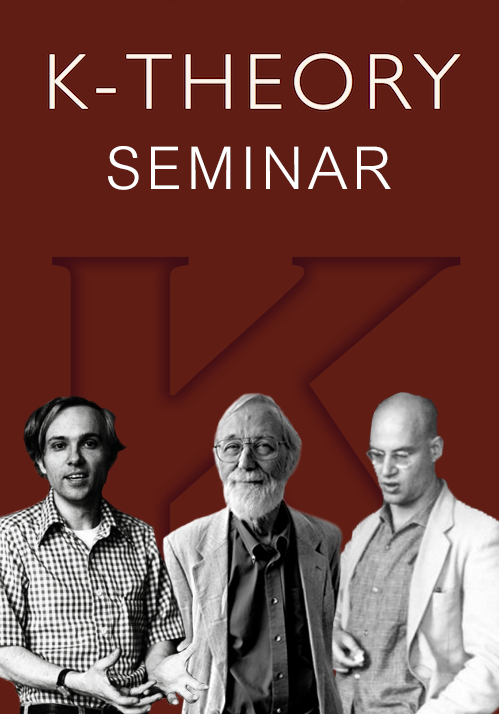
\includegraphics[width=90mm]{seminar}}\\

{\large 从左至右依次为\\
Quillen~~Milnor~~Grothendieck}\\
\vfill
% \plogo\\[0.5\baselineskip]
\today
\end{center}
\endgroup}